
% KAPITEL 3: Versuchsaufbau und Methodik (03_methodenteil.tex)


\section{Versuchsaufbau und Methodik}
\label{chap:methodik}

Dieses Kapitel erläutert die experimentelle Grundlage der vorliegenden Arbeit und dokumentiert den Prozess von der Konzeption bis zur validen Datenerfassung. Im Fokus steht der Hochstromprüfstand, welcher für die Generierung von Primärströmen \gls{sym:I_p} bis zu \SI{6000,00}{\ampere} ausgelegt ist. 

Dabei wird neben dem technischen Aufbau die kritische Analyse der initialen Messunsicherheiten sowie die daraus resultierende Optimierung der Messkette dargelegt. Die Implementierung präziser Digitalmessgeräte und einer automatisierten Prozesssteuerung bildet die Grundlage für die Erzielung reproduzierbarer Ergebnisse. Ergänzend werden die Kriterien für die Auswahl der Prüflinge sowie die konstruktiven Variationen der Leitergeometrien vorgestellt.

\subsection{Hochstromprüfstand}
\label{sec:hochstrom_pruefstand}

Der Hochstromprüfstand bildet die experimentelle Basis für die durchgeführten Untersuchungen. In diesem Abschnitt wird zunächst die technische Realisierung der Stromerzeugung sowie das digitale Regelungskonzept erläutert. Darauf aufbauend erfolgt eine Analyse der ursprünglich eingesetzten Messtechnik. Die Identifikation der dabei aufgetretenen Defizite dient als Grundlage für die im weiteren Verlauf dargelegte Optimierung des Messsystems.

Die Anlage dient der Erzeugung und Regelung hoher Wechselströme (\gls{ac}) für thermische sowie elektrodynamische Untersuchungen an elektrischen Betriebsmitteln. Als Prüflinge fungieren üblicherweise Niederspannungsschaltanlagen oder deren Teilkomponenten, die unter Lastbedingungen auf ihre thermische Belastbarkeit geprüft werden. Die Anlage ermöglicht die Bereitstellung von Strömen bis zu \SI{6000}{A} bei einer Spannung von circa \SI{6}{V}.

\subsubsection{Aufbau und Funktionsweise}
\label{sec:aufbau_funktionsweise}

Der Leistungspfad beginnt primärseitig mit einem motorbetriebenen Säulenstelltransformator der Firma \textit{Ruhstrat}, der mit einer Bemessungsleistung von \SI{90}{kVA} als zentrales Stellglied fungiert. Dem Transformator sind Netzdrosseln nachgeschaltet, welche zur Bedämpfung von Stromspitzen dienen. Die Spannungsstellung erfolgt stufenlos über verstellbare Kohlerollbürsten, wodurch eine variable Ausgangsspannung im Bereich von \SI{0}{V} bis \SI{380}{V} bereitgestellt wird.

Diese Spannung speist den nachgeschalteten Hochstrom-Festtransformator der \textit{Rolf Janssen Elektrotechnische Werke GmbH} (Typ UI 260/420 M). Mit einer Nennleistung von \SI{30}{kVA} transformiert dieser die Eingangsspannung auf eine Kleinspannung von \SI{6}{V} herab, was sekundärseitig die Realisierung von Prüfströmen \gls{sym:I_p} bis zu \SI{6000}{A} am dreiphasigen Abgang ermöglicht.

\begin{figure}[H]
    \centering
    \includegraphics[width=1.0\textwidth]{03_Ressourcen/zeichnungen/aufbau_hochstrom_pruefstand.drawio.pdf}
    \caption{Blockschaltbild des Hochstromprüfstandes mit Leistungs- und Signalpfaden}
    \label{pic:aufbau_hochstrom_pruefstand}
\end{figure}

\subsubsection{Regelungskonzept}
\label{sec:regelungskonzept}

Die Stromregelung ist als digitaler \gls{pid}-Regelkreis innerhalb des Peripheriesystems Siemens \gls{et200s} implementiert. Der Bediener definiert über die \gls{wincc}-Visualisierung den Sollstrom, welchen die \gls{sps} kontinuierlich mit dem rückgeführten Istwert vergleicht. Als Stellgröße generiert die Steuerung Schaltbefehle für den Antriebsmotor des Säulenstelltransformators.



Um hochfrequente Regelvorgänge zu vermeiden, welche transiente Stromspitzen induzieren könnten, wurde eine Hysterese in Form eines Totbandes in den Algorithmus integriert. Neben der Parametrierung der Regelstrecke übernimmt die Visualisierung die lückenlose Messwerterfassung der Versuchsverläufe. Eine detaillierte Spezifikation der eingesetzten Systemkomponenten ist in Tabelle~\ref{tab:komponenten_hochstrom} dargelegt.

\begin{table}[H]
    \centering
    \caption{Detaillierte Spezifikation der Komponenten des Hochstromprüfstands}
    \label{tab:komponenten_hochstrom}
    \small
    \begin{tabularx}{\textwidth}{@{}l l l l X@{}}
        \toprule
        \textbf{Komponente}      & \textbf{Typ}         & \textbf{\makecell[l]{Leistung /                                                                                                                   \\ Bürde}} & \textbf{\makecell[l]{Primär / \\ Input}} & \textbf{\makecell[l]{Sekundär / \\ Output}} \\ \midrule
        Säulenstelltransformator & Ruhstrat             & \SI{90}{kVA}                                                                & \SI{380}{V}                      & \SIrange{0}{380}{V} (\SI{70}{A}) \\
        Festtransformator        & Janssen              & \SI{30}{kVA}                                                                & \SI{380}{V}                      & \SI{6}{V} (\SI{5000}{A})         \\
        Stromwandler             & Celsa ICG            & \SI{5}{VA}                                                                  & \SI{6000}{A}                     & \SI{5}{A} (Kl. 0,2S)             \\
        Messumformer (3-K)       & 3-K Elektrik         & --                                                                          & \SI{0}{A} bis \SI{5}{A} \gls{ac} & \SIrange{0}{20}{mA} \gls{dc}     \\ \midrule
        \textbf{Leittechnik}     & \textbf{Typ}         & \multicolumn{3}{l}{\textbf{Beschreibung}}                                                                                                         \\ \cmidrule(r){1-2}
        Steuerung                & Siemens \gls{et200s} & \multicolumn{3}{l}{\gls{profinet}-Anbindung, Stromregelung, Analogeingänge}                                                                       \\
        Visualisierung           & Siemens \gls{wincc}  & \multicolumn{3}{l}{\gls{hmi}-System, Prozessüberwachung, Datenlogging}                                                                            \\ \bottomrule
    \end{tabularx}
\end{table}

\paragraph{Anforderungen an die Referenzmessstrecke}
\label{par:anforderungen_referenz}

Für die Durchführung der experimentellen Untersuchungen an den Stromwandlern ist die Bereitstellung einer Referenzmessstrecke erforderlich, die eine valide Bewertung gemäß der Genauigkeitsklasse \num{1,00} ermöglicht. Hierzu werden die Referenzmessmittel, die Stromerzeugung sowie die Signalführung als geschlossene Messkette ausgelegt und vorab verifiziert. 



Um die Anforderungen an ein wissenschaftliches Referenzsystem zu erfüllen, wird für die Primärstromerfassung eine deutlich höhere Präzision als die Zielklasse der Prüflinge angesetzt (z.\,B. Klasse \num{0,2} bzw. \num{0,2}S). Dadurch wird sichergestellt, dass die kombinierte Messunsicherheit der Referenzmessung hinreichend klein gegenüber den zulässigen Fehlergrenzen der Klasse \num{1,0} bleibt. Diese methodische Trennung gewährleistet, dass beobachtete Messabweichungen eindeutig den Charakteristika der Prüflinge zugeordnet werden können und keine signifikanten Einflüsse durch die Versuchseinrichtung enthalten sind.




\subsubsection{Ursprünglicher Aufbau der Messstrecke}
\label{sec:aufbau_alter_messstrecke}

Die initiale Konfiguration der Messstrecke (siehe Abbildung~\ref{pic:aufbau_messstrecke}) sah zwei parallele Erfassungspfade vor. Zur Bestimmung des Referenzwertes der Einspeisung wurden 3-K Messumformer eingesetzt, welche die Signale an die \gls{sps} übermittelten.


\begin{figure}[H]
    \centering
    \includegraphics[width=1.0\textwidth]{03_Ressourcen/zeichnungen/aufbau_messstrecke.drawio.pdf}
    \caption{Schematischer Aufbau der Messstrecke zur Ermittlung der Messabweichung}
    \label{pic:aufbau_messstrecke}
\end{figure}

Parallel dazu erfolgte die Erfassung des Sekundärsignals des Prüflings mittels eines Digitalmultimeters der Marke \textit{Fluke} im Betriebsmodus „Acquire“.




\subsubsection{Schwachstellen im Messkonzept}
\label{sec:fehleranalyse}

Die Auswertung der initialen Messreihen zeigt signifikante Abweichungen, die über den gesamten Erfassungsbereich auftreten. In Abbildung~\ref{pic:dia_messstrecke_alt} sind die Verläufe der K-3 Messumformer (blau) und der Rogowskispulen (orange) gegenübergestellt. Die Rogowskispulen wurden parallel integriert, um deren Eignung für die hochpräzise Prüfung der Wandler zu evaluieren. Beide Systeme erfassten die Messwerte zeitgleich an einem gemeinsamen Messpunkt sekundärseitig des Festtransformators.

Als Bezugssystem für die Bewertung der gesamten Messkette wird die Genauigkeitsklasse 0,2 herangezogen. Dies stellt eine konservative Betrachtung dar, da die primärseitigen Stromwandler der Klasse 0,2S entsprechen. Gemäß der Norm \cite{norm-DIN_EN_61869_2-Messwandler_Teil2-DIN} definiert die Sonderklasse 0,2S insbesondere im niedrigen Strombereich strengere Anforderungen als die Standardklasse 0,2. Da die ermittelten Abweichungen jedoch bereits die weiteren Toleranzgrenzen der Klasse 0,2 überschreiten, ist diese als Vergleichsmaßstab für die Fehleranalyse hinreichend.

Ein wesentlicher Aspekt der beobachteten Unstimmigkeiten liegt in der unterschiedlichen physikalischen Wirkweise der Sensoren begründet. Während der K-3 Messumformer als fest installierte Komponente primär Linearitätsfehler im unteren Skalenbereich aufweist, unterliegen die Rogowskispulen zusätzlich stochastischen Einflüssen durch ihre mechanische Flexibilität und die damit verbundene Lageempfindlichkeit. Da das Magnetfeld am Prüfstand durch die engen Schienenabstände stark inhomogen ist, führt bereits eine geringfügige Verkippung der Spulen zu signifikanten Fehlern im Integrationsergebnis, was die inkonsistenten Verläufe zwischen den Phasen L1 und L2 miterklärt.

\begin{diagram}[H]
    \centering
    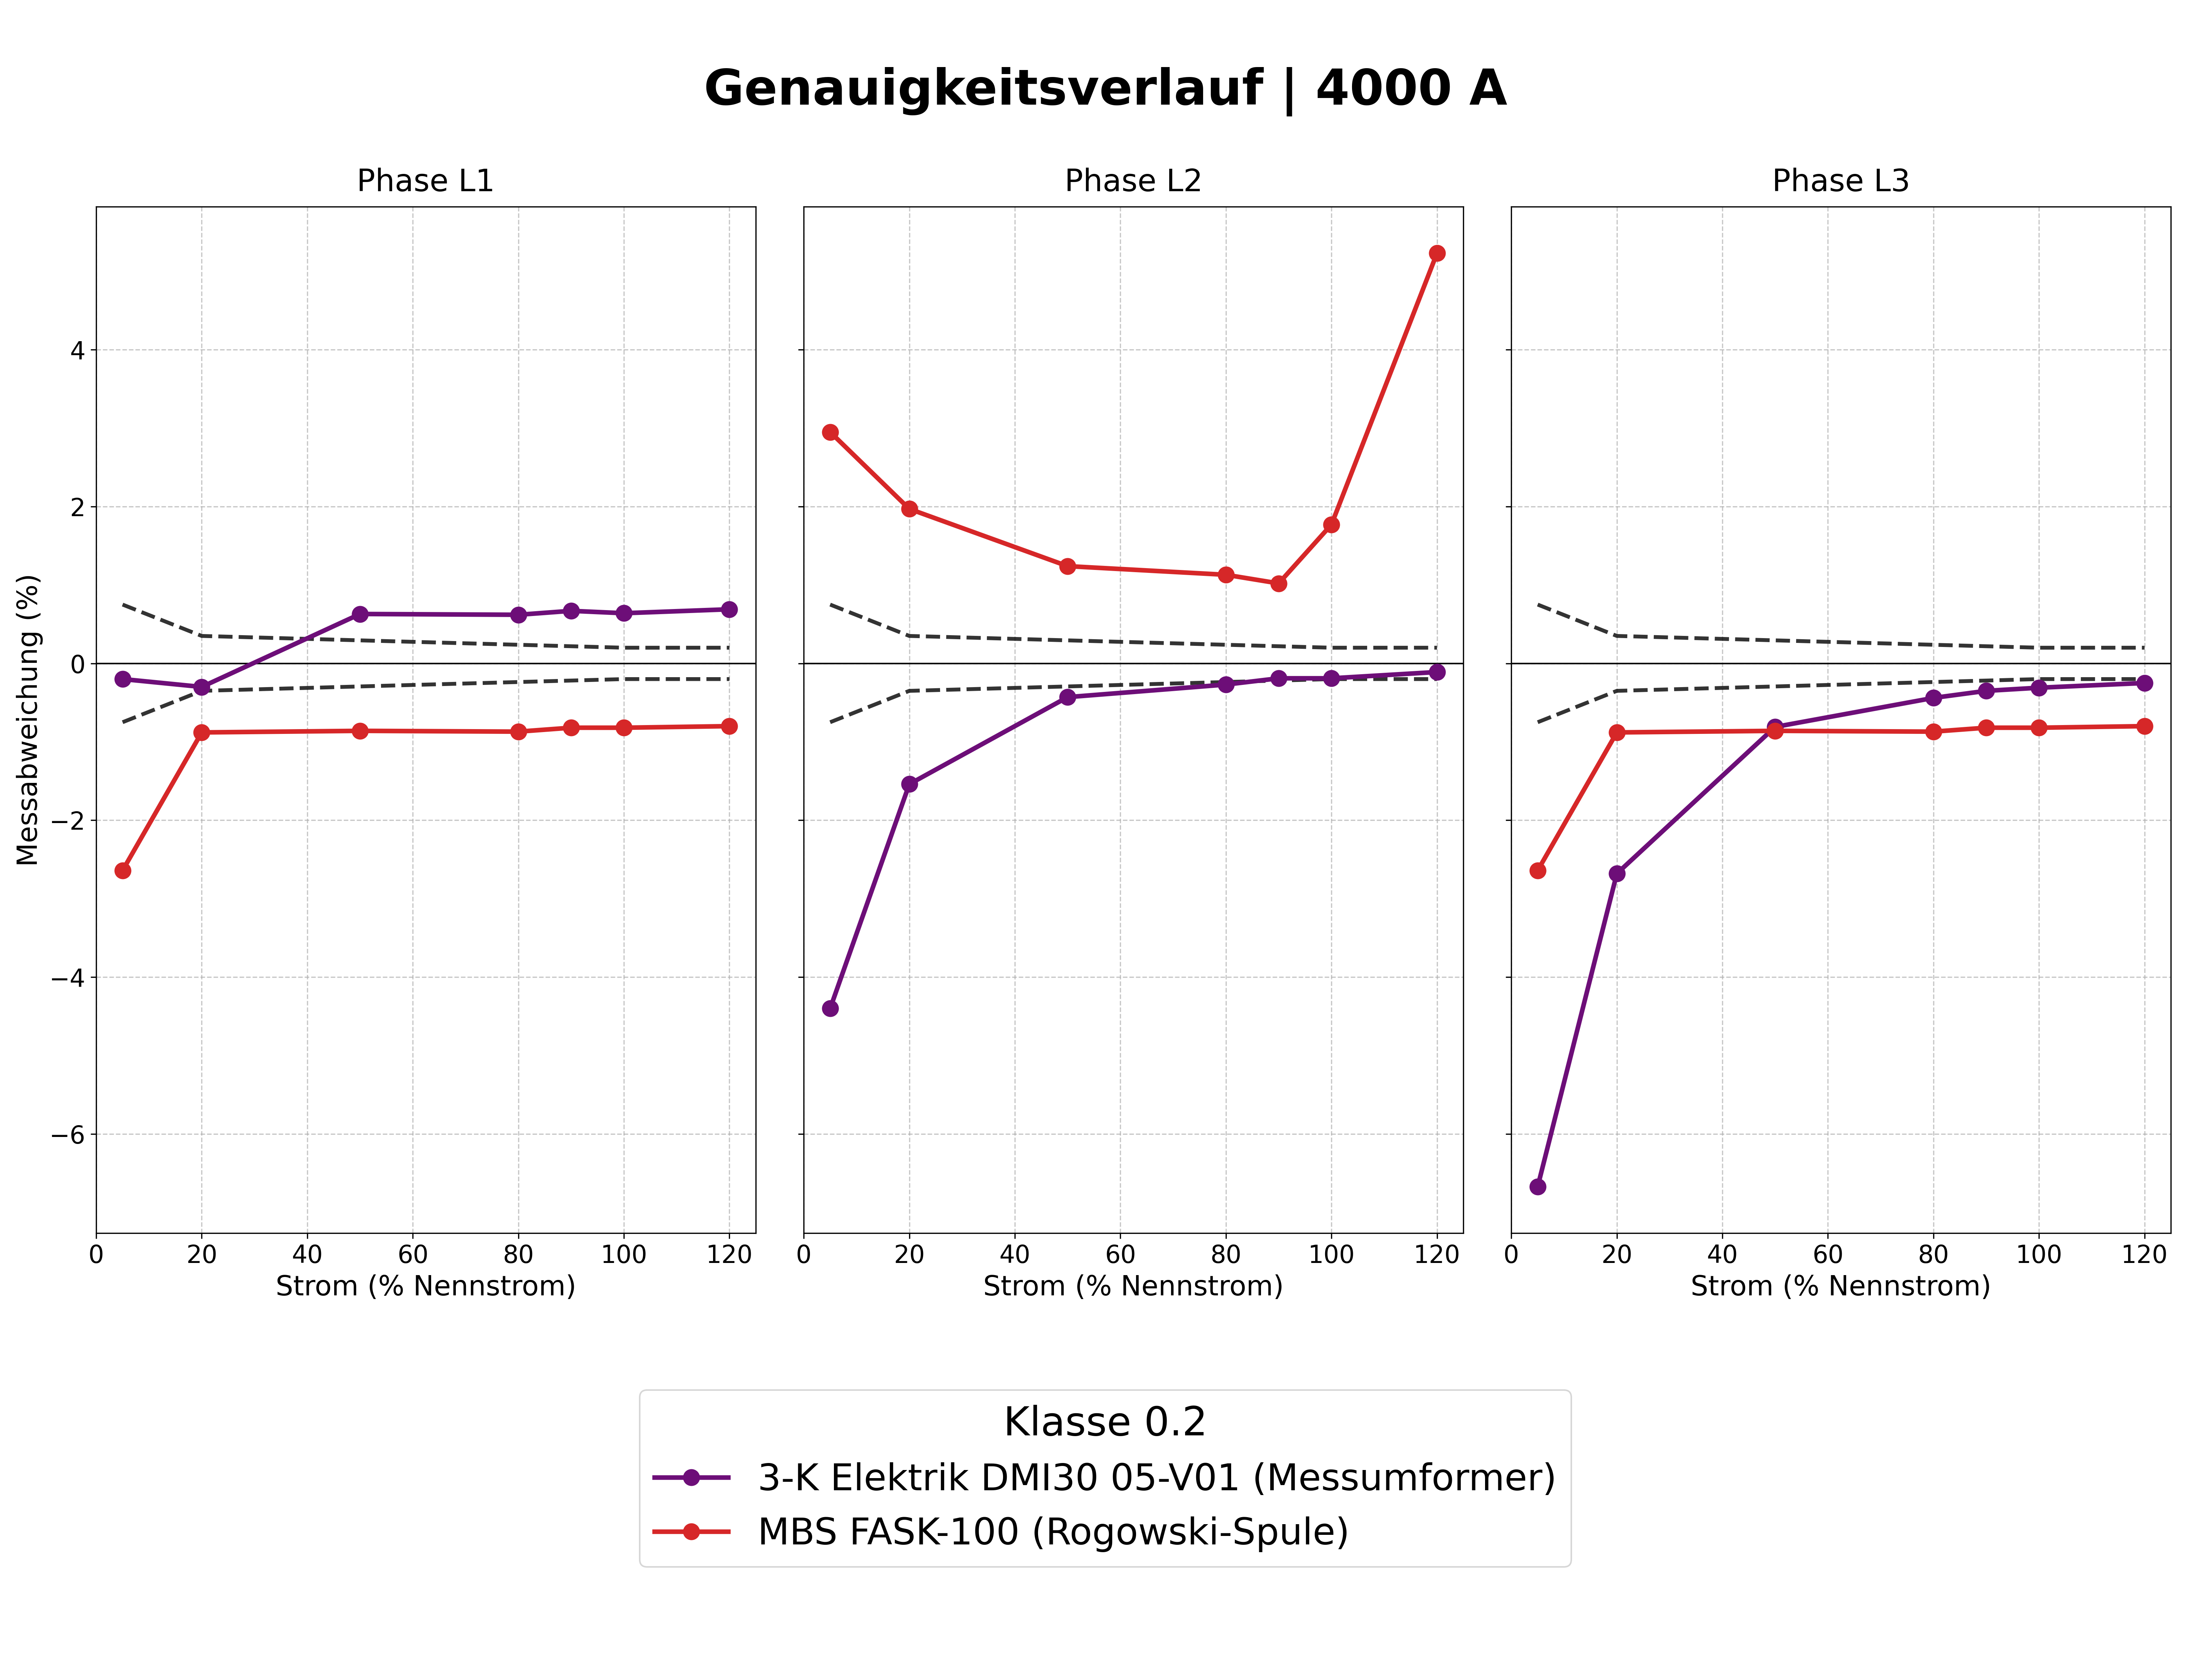
\includegraphics[width=1.0\textwidth]{03_Ressourcen/dia_neu/verlauf/mes_messstrecke_alt_verlauf.png}
    \caption{Analyse der Messabweichung und Standardabweichung der Phasen L1, L2 und L3 im ursprünglichen Versuchsaufbau}
    \label{pic:dia_messstrecke_alt}
\end{diagram}

Die grafische Darstellung verdeutlicht, dass beide Messsysteme die normativ vorgegebenen Toleranzgrenzen (gestrichelte Linien) nicht einhalten. In Phase L1 überschreitet der K-3 Messumformer ab einer Last von \SI{50}{\percent} den positiven Grenzwert, während die Rogowskispulen eine negative Abweichung zwischen \num{-1,00}\,\% und \num{-2,50}\,\% aufweisen. In Phase L2 zeigt der Messumformer bei \SI{20}{\percent} Last einen Abfall der Genauigkeit auf circa \num{-2,00}\,\%, wohingegen die Rogowskispulen eine positive Abweichung von über \num{1,00}\,\% erreichen. 



Da beide Systeme die geforderte Genauigkeitsklasse signifikant verfehlen, sind sie für eine valide Referenzmessung ungeeignet. Die vorliegenden Ergebnisse unterstreichen die Problematik, dass die Eigenfehler der verwendeten Sensorik in derselben Größenordnung liegen wie die zu untersuchenden Effekte der Prüflinge. Für eine wissenschaftlich fundierte Validierung ist jedoch ein Referenzsystem erforderlich, dessen Unsicherheit deutlich unterhalb der Toleranzgrenzen des Testobjekts angesiedelt ist. Folglich kann auf Basis dieser Komponenten kein belastbarer Referenzwert für den Primärstrom \gls{sym:I_p} bestimmt werden, was die Validierung der Prüflinge verunmöglicht.



Die im unteren Segment der Abbildung~\ref{pic:dia_messstrecke_alt} dargestellte Standardabweichung \gls{sym:sigma} verdeutlicht, dass beide Messgeräte im niedrigen Strombereich eine erhöhte Varianz aufweisen. Dies ist darauf zurückzuführen, dass der Säulenstelltransformator bei geringen Strömen einen begrenzten Stellbereich besitzt, woraus eine instabile Regelung des Istwertes resultiert. Mit zunehmender Stromstärke \gls{sym:I_p} reduziert sich dieses Signalrauschen deutlich. Dabei weisen die K-3 Messumformer eine geringere Schwankungsbreite auf als die Rogowskispulen. Aufgrund dieser Defizite ist die initiale Messkette für die angestrebte Genauigkeitsprüfung unzureichend. Im folgenden Abschnitt \ref{sec:optimierung_messsystem} wird die Systemoptimierung erläutert, um eine präzisere Messwerterfassung zu realisieren.



\subsection{Optimiertes Messsystem}
\label{sec:optimierung_messsystem}

Wie im vorangegangenen Abschnitt dargelegt, erfüllte die initiale Messstrecke nicht die Anforderungen an eine präzise Genauigkeitsprüfung von Messstromwandlern. Aus diesem Grund wurde eine umfassende Optimierung des Hochstromprüfstandes durchgeführt. Das primäre Ziel dieser Maßnahmen war die Steigerung der Messgenauigkeit sowie die Automatisierung des Prüfablaufs, um reproduzierbare und unmittelbar vergleichbare Ergebnisse sicherzustellen.

Zur technischen Umsetzung wurden zwei digitale Energiemessgeräte der Siemens-Produktfamilie ausgewählt. Das Modell \gls{pac} 3220, welches für die Erfassung des Prüflingsstroms eingesetzt wird \cite[S.~97]{pdf-Handbuch_PAC3120-Siemens}, sowie das zur Überwachung der Einspeisung genutzte \gls{pac} 4220 \cite[S.~94]{pdf-Handbuch_PAC4220-Siemens}, verfügen jeweils über die Genauigkeitsklasse 0,2 für die Strommessung. 

\begin{figure}[H]
    \centering
    \includegraphics[width=1.0\textwidth]{03_Ressourcen/zeichnungen/aufbau_hochstrom_pruefstand_new.drawio.pdf}
    \caption{Schematischer Aufbau der optimierten Messstrecke mit Siemens SENTRON Messgeräten}
    \label{pic:aufbau_messstrecke_neu}
\end{figure}

Diese Geräte ermöglichen durch optionale Erweiterungsmodule eine direkte Integration in die Systemumgebung der Siemens \gls{et200s} via \gls{profinet}-Protokoll. Ein wesentlicher Vorteil dieser Konfiguration liegt in der dezentralen Messwerterfassung unmittelbar am Messpunkt. Dadurch lassen sich parasitäre Effekte über lange Messleitungen effektiv reduzieren. Die Einbindung in die \gls{sps} erfolgt durch eine direkte zyklische Datenübertragung, wodurch die manuelle Abfrage von Registern entfällt und eine zeitsynchrone Datenbasis für beide Messpunkte geschaffen wird.



Die in Abbildung~\ref{pic:aufbau_messstrecke_neu} dargestellte Systemarchitektur verdeutlicht die informationstechnische Vernetzung des optimierten Messaufbaus. Während der obere Teil des Schemas den bereits beschriebenen Leistungspfad darstellt, erfolgt die messtechnische Erfassung der Primärströme \gls{sym:I_p} zyklisch durch die Geräte \gls{pac} 4220 (Einspeisung) und \gls{pac} 3220 (Prüfling). Die erfassten Stromwerte werden in \gls{wincc} archiviert und stehen dort für die Prozessüberwachung zur Verfügung. Über die Benutzeroberfläche (\gls{hmi}) können diese Daten als \gls{csv}-Datei exportiert werden. Diese Datei dient als Grundlage für die anschließende Genauigkeitsmessung und die detaillierte Auswertung der Versuchsreihen.

\subsubsection{Softwaregestützte Prozesskette zur Datenauswertung}
\label{sec:datenaufbereitung_analyse}

Die vom Prüfstand exportierten Rohdaten liegen im \gls{csv}-Format vor und enthalten die zeitlichen Verläufe der Ströme \gls{sym:I_p} (Referenz) und \gls{sym:I_sec} (Prüfling). Angesichts des Umfangs der Untersuchung, die 31 Konfigurationen mit jeweils zwei Messgeräten und drei Phasen umfasst, ergaben sich insgesamt über 180 auszuwertende Einzelmessreihen. Eine manuelle Verarbeitung dieser Datenmenge mittels Tabellenkalkulation wäre aufgrund des hohen Zeitaufwands und der Fehleranfälligkeit bei manuellen Übertragungen unzweckmäßig. Aus diesem Grund wurde eine spezialisierte Auswertungssoftware auf Basis von \textit{Python} entwickelt.



\paragraph{Extraktion und Filterung der Messdaten}

Der erste Prozessschritt der Auswertung erfolgt im Modul \textit{„Manueller~Rohdaten-Export“} (siehe Abbildung~\ref{pic:manual_tagger}). Da die Datenerfassung am Prüfstand mit einer Abtastrate von \SI{2}{Hz} erfolgt, entstehen umfangreiche Zeitreihen. Die zentrale Funktion des Rohdaten-Selektors besteht darin, die aufgezeichneten Laststufen zu analysieren und die stationären Messbereiche zu isolieren. Hierbei werden die transienten Ein- und Ausschwingvorgänge aus dem Datensatz entfernt, sodass ausschließlich die stabilen Phasen in die weiterführende Genauigkeitsberechnung einfließen.

\begin{figure}[H]
    \centering
    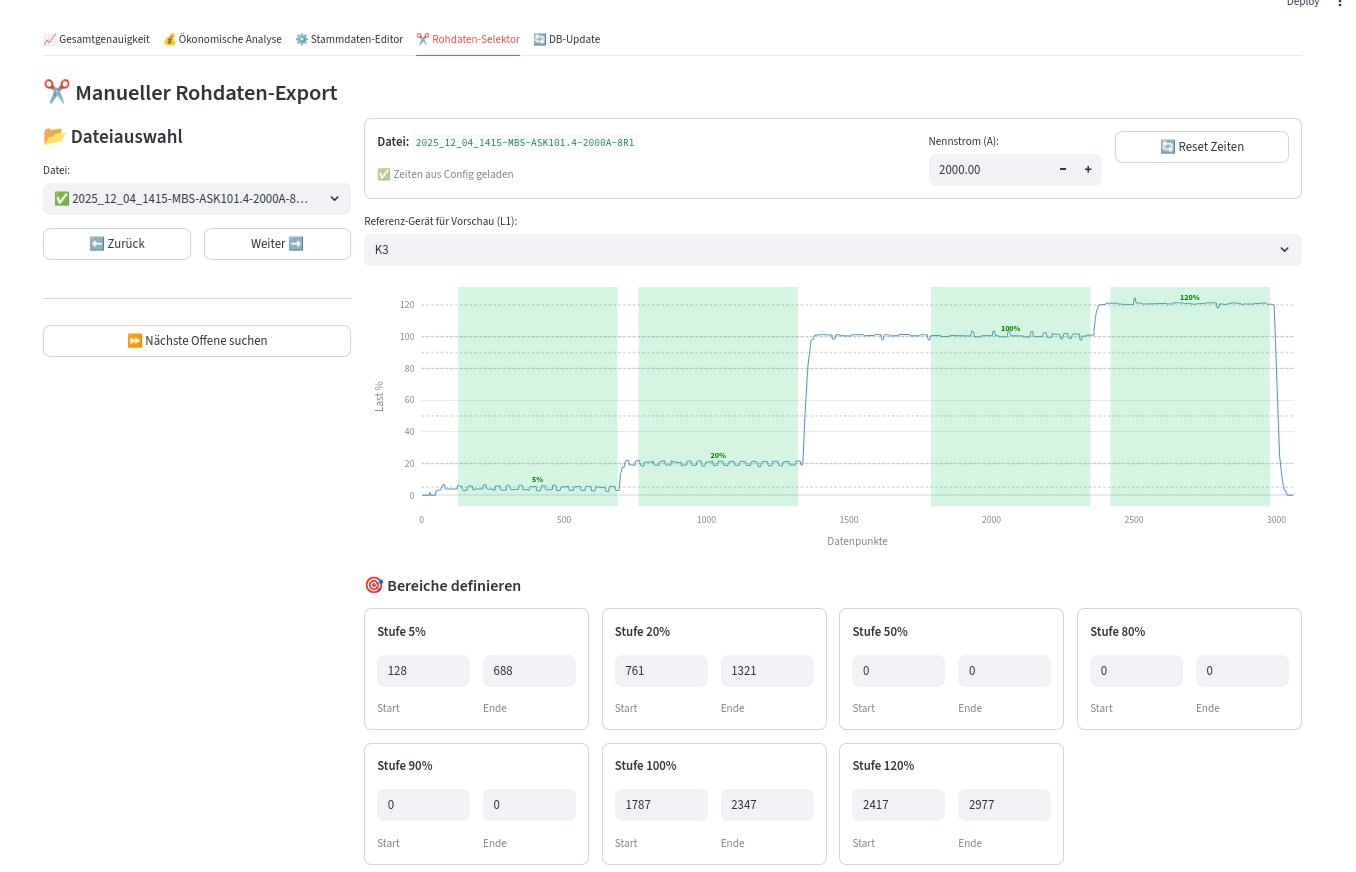
\includegraphics[width=1.0\textwidth]{03_Ressourcen/pdf/datenverarbeitung/rohdaten_export.png}
    \caption{Benutzeroberfläche des manuellen Rohdaten-Exports zur Selektion stabiler Messbereiche}
    \label{pic:manual_tagger}
\end{figure}

Für die Berechnung werden pro Laststufe exakt 560 Messpunkte herangezogen, was einem Zeitfenster von 4 Minuten und 40 Sekunden entspricht. Obwohl das Plateau technisch fünf Minuten gehalten wird, werden die letzten 20 Sekunden des Datensatzes verworfen. Diese Maßnahme dient als Sicherheitsabstand, um sicherzustellen, dass keine Signalflanken des Abschaltvorgangs in die Berechnung einfließen. Die verbleibenden 560 Werte bilden eine statistisch valide Basis für die Auswertung. Die selektierten Bereiche werden als sortierte Datensätze in der Datenbank persistiert.

\paragraph{Mathematische Berechnung}

Die mathematische Grundlage für die in der Software ermittelten Kennwerte bildet die Berechnung der prozentualen Übersetzungsmessabweichung \gls{sym:epsilon} gemäß Abschnitt \ref{sec:messabweichung_kenngroessen}. Für die automatisierte Auswertung werden zunächst die arithmetischen Mittelwerte der Ströme über das stabile Zeitfenster gebildet und anschließend verrechnet:



\begin{equation}
    \label{eq:messabweichung_allg}
    \varepsilon = \frac{\bar{I}_{s} - \bar{I}_{pri}}{\bar{I}_{pri}} \cdot 100\,\%
\end{equation}

Als Bewertungsgröße wird in dieser Arbeit ausschließlich die Übersetzungsmessabweichung \gls{sym:epsilon} ausgewertet; eine Fehlwinkelbestimmung \gls{sym:deltaphi} erfolgt nicht.


Hierbei beschreibt $\bar{I}_{s}$ den arithmetischen Mittelwert der gemessenen Stromstärke des Prüflings und $\bar{I}_{pri}$ den Mittelwert des Referenzmessgerätes im identischen Zeitraum. Ergänzend hierzu berechnet die Software die Standardabweichung \gls{sym:sigma} auf Basis der Einzelmesswerte $x_i$, um die Signalstabilität innerhalb des Plateaus zu quantifizieren:

\begin{equation}
    \label{eq:standardabweichung}
    \sigma = \sqrt{\frac{1}{N-1} \sum_{i=1}^{N} (x_i - \bar{x})^2}
\end{equation}

Diese statistische Kenngröße dient als Indikator für die Güte der Regelung und die Ruhe des Messsignals.

\paragraph{Analyse und Visualisierung}

Nach Abschluss der Berechnungen stehen die Ergebnisse in zwei spezialisierten Analyse-Modulen zur Verfügung. Der Reiter \textbf{„Gesamtgenauigkeit“} ermöglicht den detaillierten technischen Vergleich. Hier wird die prozentuale Messabweichung \gls{sym:epsilon} über dem Primärstrom \gls{sym:I_p} aufgetragen. Die Darstellung ist frei konfigurierbar, sodass verschiedene Wandlertechnologien oder Messreihen visuell mit den normativen Fehlergrenzen (z.\,B. Klasse \num{1}) verglichen werden können.

Für eine bewertende Übersicht dient der Reiter \textbf{„Ökonomische Analyse“}. Um die Komplexität der Kennlinien für einen direkten Vergleich zu reduzieren, aggregiert die Software die Messabweichungen in drei signifikante Betriebsbereiche:

\begin{itemize}
    \item \textbf{Nennstrombereich:} Erfasst das Anlaufverhalten und die Genauigkeit bei geringer Last (z.\,B. \SI{5}{\percent} und \SI{20}{\percent} \gls{sym:In}).
    \item \textbf{Nennstrombereich:} Bildet den Hauptarbeitsbereich um den Nennstrom ab (z.\,B. \SI{50}{\percent} bis \SI{100}{\percent} \gls{sym:In}).
    \item \textbf{Überstrombereich:} Visualisiert das Verhalten bei Überlast (z.\,B. \SI{120}{\percent} \gls{sym:In}).
\end{itemize}

Um für diese Bereiche einen einzelnen vergleichbaren Gütefaktor zu erhalten, werden die prozentualen Messabweichungen \gls{sym:epsilon} der zugehörigen Lastpunkte aggregiert. Hierfür wird der arithmetische Mittelwert der Absolutbeträge gebildet. Dies verhindert, dass sich positive und negative Abweichungen (z.\,B. $+\num{0,50}\,\%$ und $-\num{0,50}\,\%$) gegenseitig kompensieren:

\begin{equation}
    \label{eq:fehler_bereich}
    \bar{\varepsilon}_{\text{Bereich}} = \frac{1}{k} \sum_{j=1}^{k} |\varepsilon_j|
\end{equation}

Dabei ist $k$ die Anzahl der angefahrenen Lastpunkte innerhalb des definierten Bereichs und $|\varepsilon_j|$ der Betrag der Messabweichung am jeweiligen Prüfpunkt. In dieser Ansicht werden zudem konstruktive und wirtschaftliche Parameter wie das Gehäusevolumen und der Preis der Wandler den aggregierten Genauigkeitswerten gegenübergestellt. Dies ermöglicht eine multidimensionale Bewertung der Prüflinge hinsichtlich ihres Preis-Leistungs-Verhältnisses.

\subsubsection{Auswertung der neuen Messstrecke}
\label{sec:auswertung_messstrecke}

Die Validierung der optimierten Messstrecke belegt eine signifikante Steigerung der Messgüte im Vergleich zu den initialen Komponenten. In Abbildung~\ref{dia:messstrecke_neu} ist der Fehlerverlauf des neu installierten Energiemessgerätes \gls{pac} 4220 (magenta) im direkten Vergleich zum Messumformer 3-K (grün) und den Rogowskispulen (blau) dargestellt. 



Der Kurvenverlauf verdeutlicht, dass das \gls{pac} 4220 über nahezu den gesamten Lastbereich innerhalb des normativen Toleranzbandes der Genauigkeitsklasse \num{0,2} verbleibt. Ab einer Last von \SI{20}{\percent} des Nennstroms \gls{sym:In} stabilisiert sich die Übersetzungsmessabweichung \gls{sym:epsilon} nahe der Nulllinie.

\begin{diagram}[H]
    \centering
    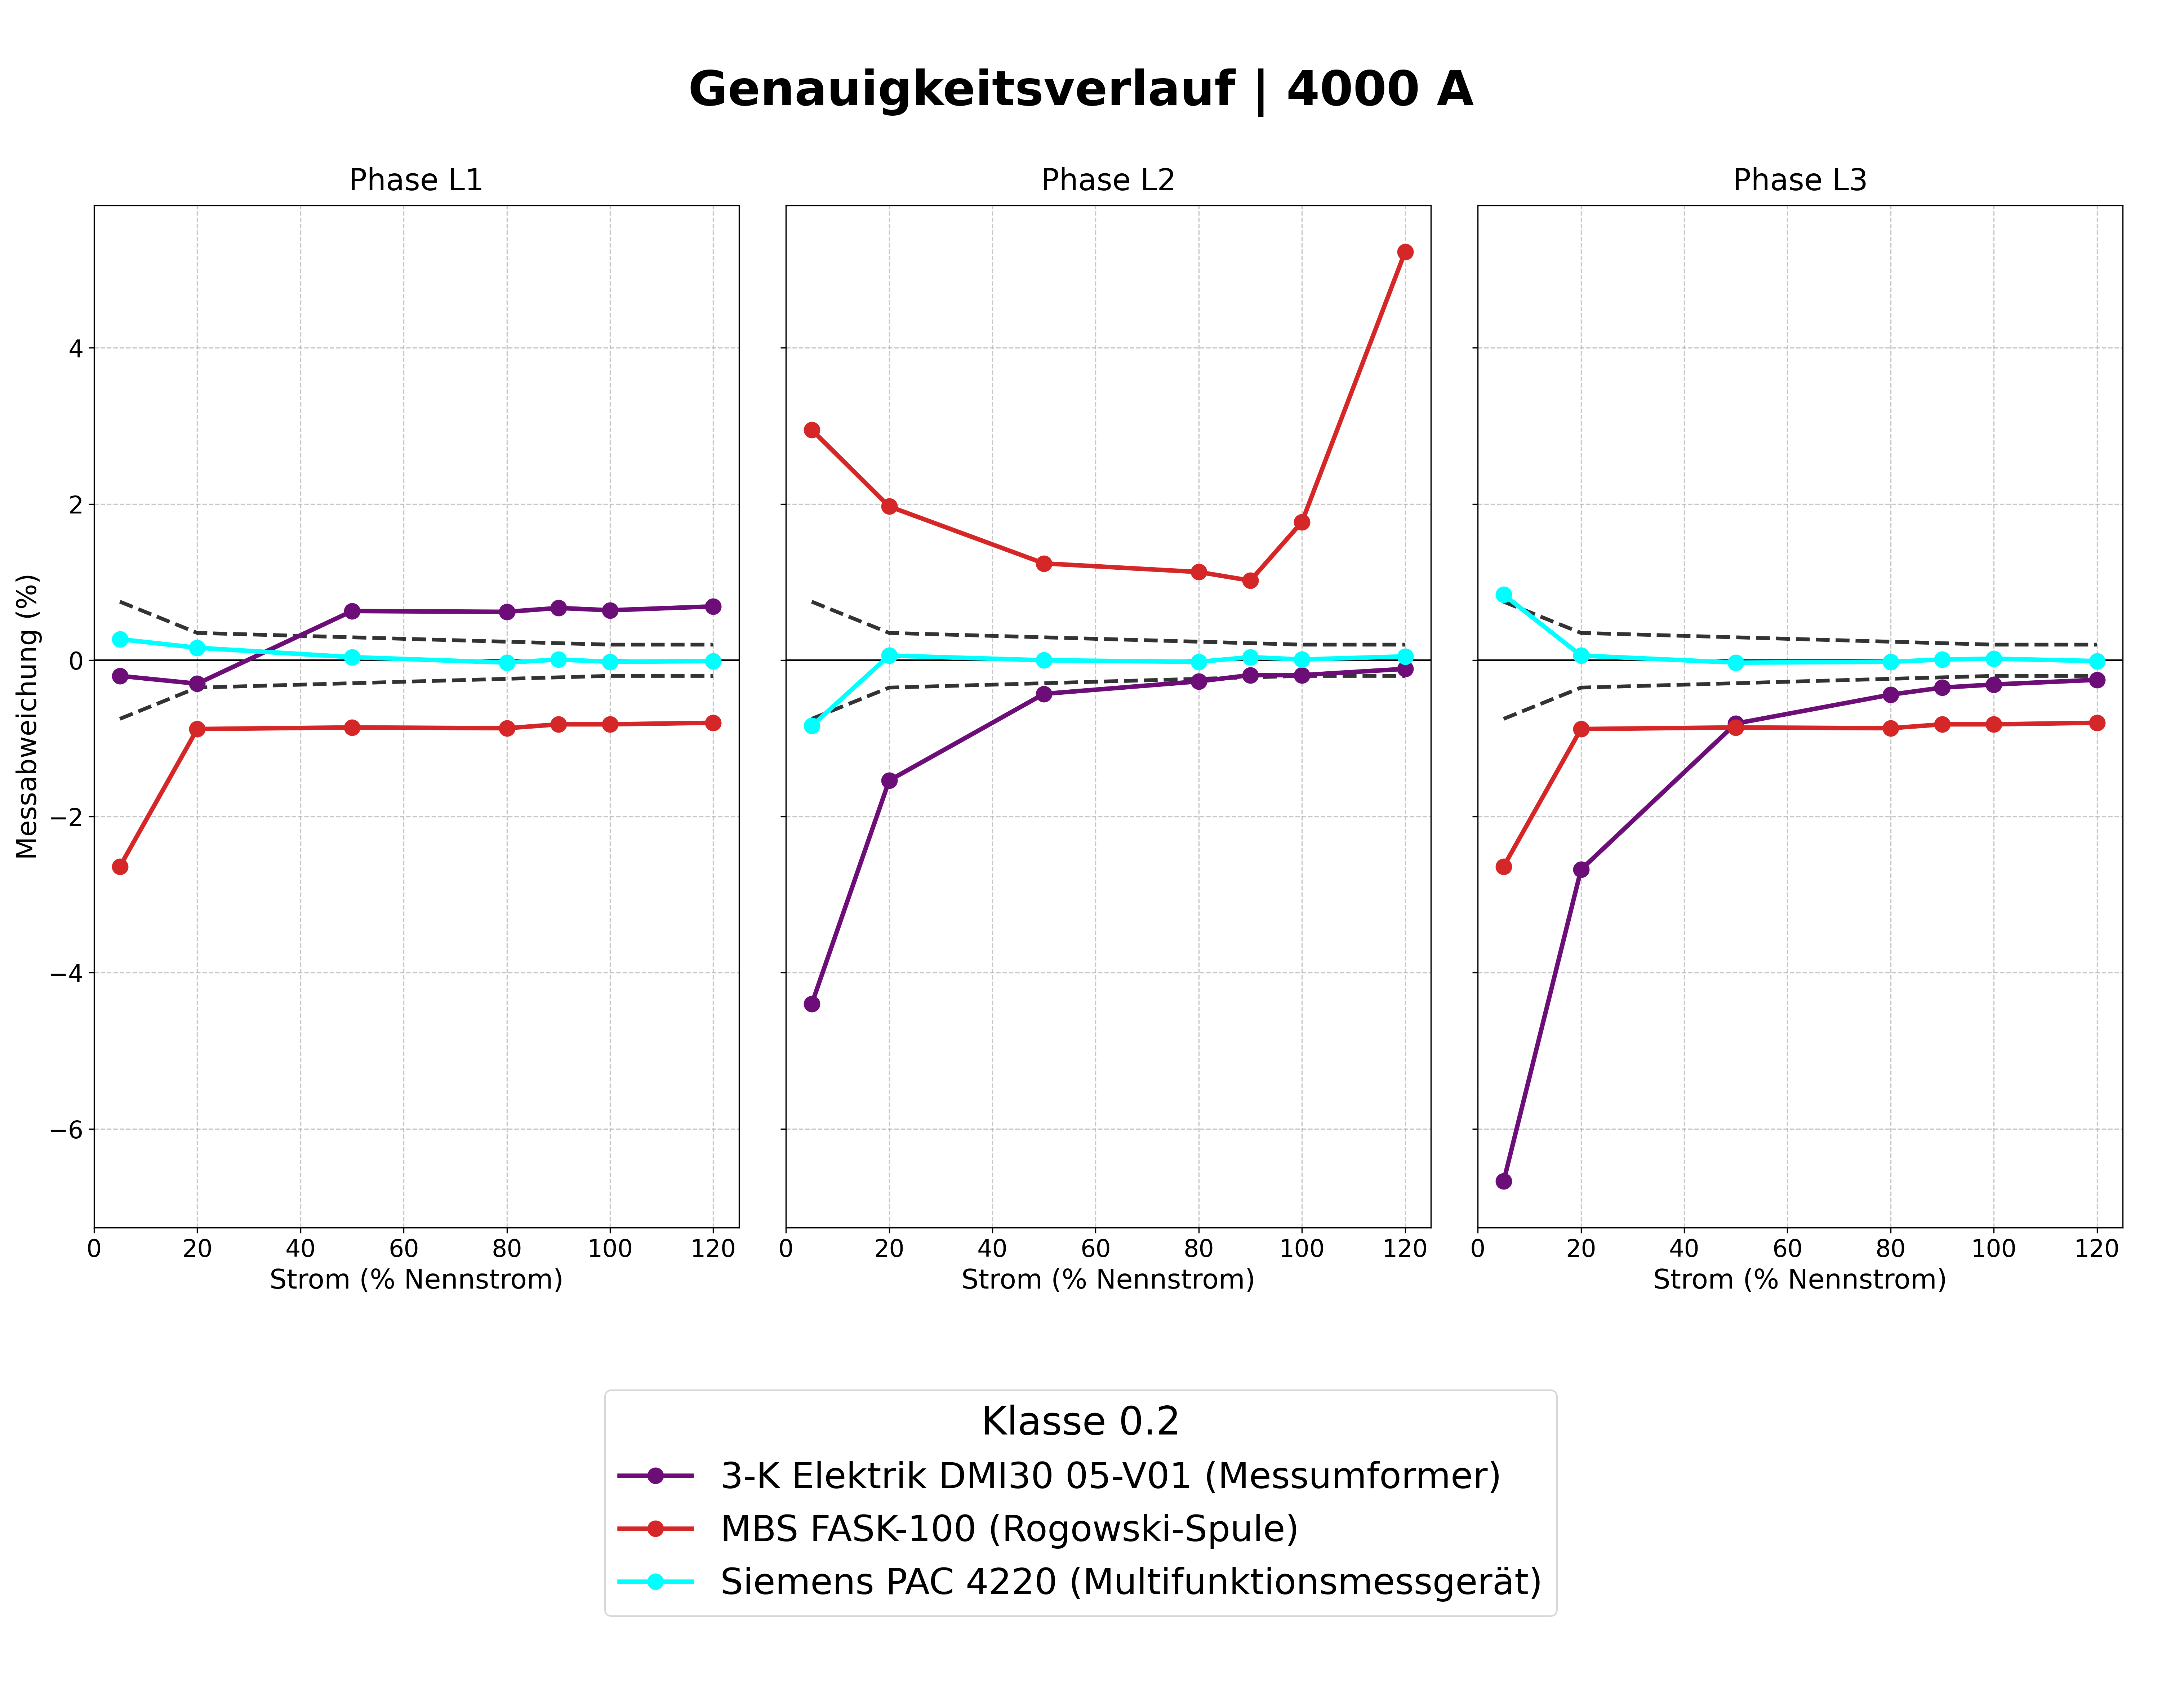
\includegraphics[width=1.0\textwidth]{03_Ressourcen/dia_neu/verlauf/mes_messstrecke_neu_verlauf.png}
    \caption{Vergleichende Analyse der Messabweichung (oben) und Standardabweichung (unten) unter Einsatz des \gls{pac} 4220}
    \label{dia:messstrecke_neu}
\end{diagram}

Eine Abweichung außerhalb der Normgrenzen ist lediglich im Bereich geringer Ströme (\SI{5}{\percent}) erkennbar. Wie in Abschnitt \ref{sec:fehleranalyse} erläutert, resultiert dieser Effekt aus dem begrenzten Stellbereich des Säulenstelltransformators, der bei minimaler Auslenkung keine stabile Stromvorgabe ermöglicht. Durch die hohe Auflösung des \gls{pac} 4220 lässt sich diese physikalische Grenze des Prüfstandes messtechnisch präzise erfassen.

Die im unteren Segment der Abbildung~\ref{dia:messstrecke_neu} visualisierte Standardabweichung \gls{sym:sigma} dient als Maß für die Präzision und Reproduzierbarkeit der Messsysteme. Hierbei weisen das \gls{pac} 4220 und der Messumformer 3-K ein ähnliches Verhalten mit einer sehr geringen Streuung auf. Ab einer Last von \SI{50}{\percent} sinkt die Standardabweichung \gls{sym:sigma} für beide Geräte auf ein Niveau von unter \num{0,50}\,\%. Im Gegensatz dazu zeigen die Rogowskispulen über den gesamten Messbereich eine deutlich höhere Streuung. Obwohl die 3-K-Umformer eine vergleichbare Präzision wie das \gls{pac}-Messgerät erzielen, verbleiben sie aufgrund ihrer hohen systematischen Abweichung außerhalb der geforderten Genauigkeitsklasse.

Ergänzend zur Analyse der Einzelabweichungen ermöglicht das Ökonomie-Ranking in Abbildung~\ref{dia:oekonomie_ranking} eine zusammenfassende Bewertung der Messsysteme.



\begin{diagram}[H]
    \centering
    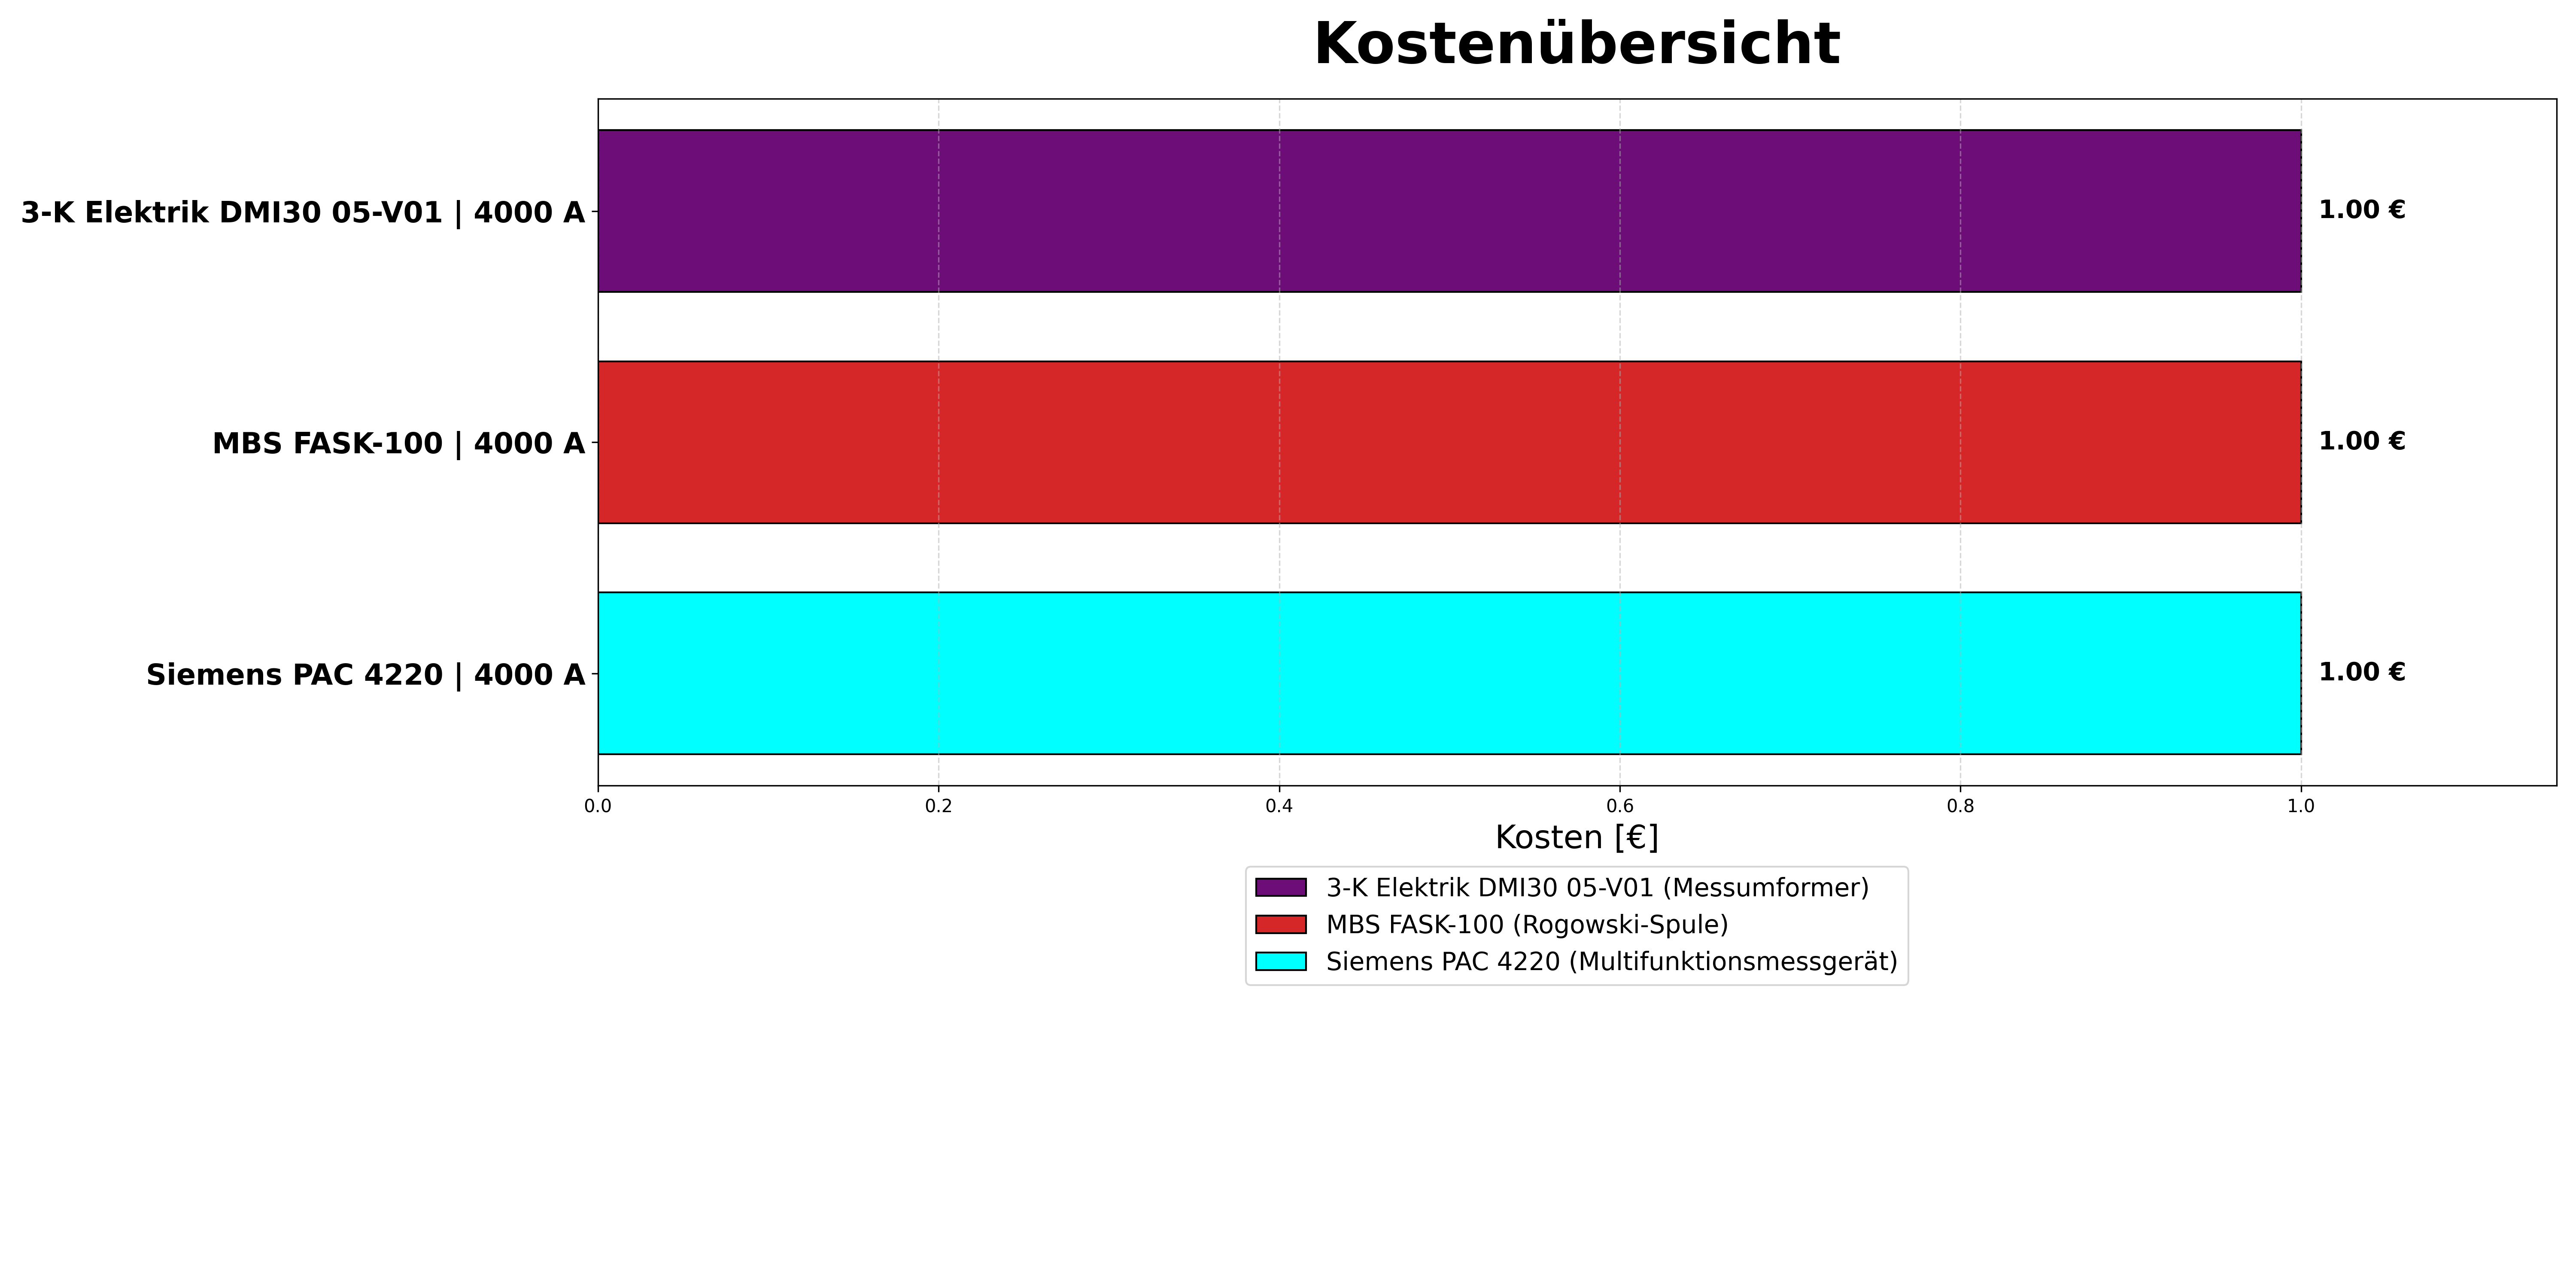
\includegraphics[width=1.0\textwidth]{03_Ressourcen/dia_neu/kosten_horizontal/mes_messstrecke_neu_kosten_horizontal.png}
    \caption{Kumulierter Vergleich der Fehleranteile (Ökonomie-Ranking) der verschiedenen Messsysteme über drei Lastbereiche}
    \label{dia:oekonomie_ranking}
\end{diagram}

Hierbei werden die kumulierten Fehleranteile in den Bereichen Niederstrom (blau), Nennstrom (rot) und Überlast (gelb) gegenübergestellt. Zur quantitativen Bewertung dieser Anteile dient der in Tabelle~\ref{tab:fehler_score_vergleich} ausgewiesene Fehler-Score. Um die unterschiedlichen Messsysteme vergleichbar zu machen, erfolgt eine Normierung der Fehlerwerte innerhalb jedes Lastbereichs. Das System mit der größten mittleren Abweichung $\bar{\varepsilon}$ im jeweiligen Bereich wird als Referenz für \SI{100,00}{\percent} gesetzt, während die anderen Systeme relativ dazu skaliert werden. Der Gesamtwert (Fehler-Score) berechnet sich anschließend aus der Summe dieser normierten Einzelwerte gemäß der Formel:

\begin{equation}
    \text{Score} = \sum_{\text{Bereich}} \left( \frac{\bar{\varepsilon}_{\text{System}}}{\bar{\varepsilon}_{\text{max}}} \cdot \SI{100,00}{\percent} \right)
\end{equation}

Ein niedriger Gesamtscore indiziert dabei eine hohe Genauigkeit über alle Betriebsbereiche hinweg.

\begin{table}[H]
    \centering
    \caption{Vergleichende Übersicht der normierten Fehleranteile und des resultierenden Fehler-Scores}
    \label{tab:fehler_score_vergleich}
    \begin{tabular}{lcccc}
        \toprule
        \textbf{Messsystem} & \textbf{Niederstrom [\%]} & \textbf{Nennstrom [\%]} & \textbf{Überlast [\%]} & \textbf{Fehler-Score [\%]} \\ 
        \midrule
        \gls{pac} 4220      & \num{13,10}               & \num{2,00}              & \num{0,96}             & \num{16,06}                \\
        3-K                 & \num{100,00}              & \num{41,19}             & \num{15,36}            & \num{156,55}               \\
        Rogowskispulen      & \num{84,50}               & \num{100,00}            & \num{100,00}           & \num{284,50}               \\ 
        \bottomrule
    \end{tabular}
\end{table}

Im direkten Vergleich erreicht das \gls{pac} 4220 einen Fehler-Score von lediglich \num{16,06}\,\%. Dies bedeutet, dass seine kumulierte Abweichung nur einen Bruchteil der Fehler der anderen Systeme beträgt. Der Messumformer 3-K weist einen kumulierten Anteil von \num{156,55}\,\% auf, da er insbesondere im Niederstrombereich die größte Ungenauigkeit aufwies und dort den \num{100,00}\,\%-Referenzwert bildete. Die Rogowskispulen markieren mit \num{284,50}\,\% die größte Gesamtabweichung, da sie im Nennstrom- und Überlastbereich jeweils die schlechtesten Ergebnisse lieferten. Diese Resultate bestätigen, dass erst durch den Einsatz der digitalen \gls{pac}-Messgeräte eine valide Datenbasis für die weitere Untersuchung geschaffen wurde.

\subsubsection{Auswahl und Spezifikation der Messstromwandler}
\label{sec:auswahl_wandler}

Für die experimentellen Untersuchungen werden Stromwandler der Hersteller \textit{MBS}, \textit{Celsa} und \textit{Redur} eingesetzt. Die Auswahl deckt ein Spektrum von marktüblichen Standardwandlern bis hin zu spezialisierten Modellen mit integriertem Fremdfeldschutz ab. Ziel dieser Zusammenstellung ist es, eine belastbare Datenbasis für die Analyse der Beeinflussungseffekte unter verschiedenen technologischen Voraussetzungen zu schaffen. 

Tabelle~\ref{tab:wandler_spezifikationen_erweitert} fasst die technischen Kenndaten der Prüflinge zusammen. Neben dem Bemessungsstrom \gls{sym:In} und der Bemessungsleistung \gls{sym:Sn} ist das Gehäusevolumen aufgeführt. Dieses dient als Vergleichsgröße für die Wirtschaftlichkeitsbetrachtung und errechnet sich aus dem Produkt der maximalen äußeren Gehäusedimensionen (Höhe $\times$ Breite $\times$ Tiefe). 



Es ist anzumerken, dass es sich hierbei um eine Vereinfachung handelt, die den Wandler auf seinen quaderförmigen Hüllkörper reduziert. Spezifische Geometrien, wie etwa Verjüngungen oder Abrundungen am Gehäuse, werden in dieser Berechnung vernachlässigt, sodass das tatsächliche Materialvolumen geringer ausfallen kann. Für die konstruktive Bewertung in Schaltanlagen ist diese Betrachtungsweise jedoch maßgeblich, da für die Montageplanung der maximale Platzbedarf (Bauraum) reserviert werden muss, den der Wandler im Anschlussraum effektiv beansprucht.

\begin{table}[H]
    \centering
    \caption{Erweiterte Spezifikationen und wirtschaftliche Kennwerte der Prüflinge nach Technologie gruppiert}
    \label{tab:wandler_spezifikationen_erweitert}
    \small
    \begin{tabular}{@{}lll S[table-format=4.0] S[table-format=2.1] S[table-format=4.2] S[table-format=3.2]@{}}
        \toprule
        \textbf{Hersteller} & \textbf{Typ} & \textbf{Technologie} & {\textbf{\gls{sym:In} [\unit{A}]}} & {\textbf{\gls{sym:Sn} [\unit{VA}]}} & {\textbf{Volumen [\unit{cm^3}]}} & {\textbf{Preis [\text{\euro}]}} \\
        \midrule
        Celsa & ALO 10030     & Standard    & 2000 & 2,5  & 634,30  & 45,50  \\
        MBS   & ASK 101.4     & Standard    & 2000 & 10,0 & 733,20  & 43,67  \\
        Celsa & ALO 10030     & Standard    & 2500 & 2,5  & 634,30  & 45,50  \\
        Celsa & ALO 12070     & Standard    & 3000 & 15,0 & 1520,00 & 71,51  \\
        Celsa & ALO 12070     & Standard    & 4000 & 15,0 & 1520,00 & 71,51  \\
        \addlinespace
        Celsa & ALO 8030 K    & Kompensiert & 2000 & 10,0 & 710,20  & 95,95  \\
        Celsa & ALO 10050 K   & Kompensiert & 2500 & 5,0  & 1027,00 & 104,20 \\
        Celsa & ALO 12070 K   & Kompensiert & 3000 & 15,0 & 1520,00 & 346,06 \\
        Celsa & ALO 12070 K   & Kompensiert & 4000 & 15,0 & 1520,00 & 401,91 \\
        \addlinespace
        Redur & 13A1030.3ffp  & \glsentryshort{ffp}   & 2000 & 10,0 & 778,70  & 146,01 \\
        \bottomrule
    \end{tabular}
\end{table}
Die eingesetzten Wandler lassen sich technologisch in drei Kategorien unterteilen. Als Basis dienen Standardwandler, die einen klassischen Aufbau ohne zusätzliche konstruktive Schutzmaßnahmen gegen externe Felder aufweisen (siehe Abschnitt \ref{sec:aufbau_wandler}). Eine weiterführende Bauform stellen die kompensierten Wandler dar. Diese Modelle verfügen über eine modifizierte Wicklungsanordnung, die gezielt zur Reduktion von Messabweichungen bei asymmetrischer Primärleiterlage eingesetzt wird (siehe Abschnitt \ref{sec:kompensationswicklungen}). 

Die dritte Gruppe bilden die spezialisierten \gls{ffp}-Wandler der Firma \textit{Redur}, welche die Technologie der Fremdfeldprotektoren nutzen. Die Schirmwirkung wird hierbei durch die Integration eines Werkstoffs mit hoher magnetischer Permeabilität realisiert. Diese Schirmung fungiert als magnetischer Shunt, der die Feldlinien benachbarter Leiter um den Messkern herumleitet. 



Infolgedessen bleibt die magnetische Induktion im Kernmaterial weitgehend unbeeinflusst von äußeren Feldern \cite{pdf-Fremdfeldstoerungen_Stromwandler-Redur}. Um die Vergleichbarkeit der Messergebnisse zu gewährleisten, entsprechen alle ausgewählten Wandler der Genauigkeitsklasse \num{1}. Die in der Tabelle aufgeführten Nennbürden sind so gewählt, dass sie die Anforderungen für die thermische Dauerbelastung erfüllen.

\subsubsection{Geometrische Anordnung der Primärleiter}
\label{sec:layout_geometrie}

In Niederspannungsschaltanlagen werden Kupferschienen vorwiegend parallel angeordnet. Diese Bauweise zeichnet sich durch hohe Platzersparnis sowie eine geringe Montagekomplexität aus. Die Führung der Schienen wird konstruktiv maßgeblich durch die Anschlussebene des Leistungsschalters determiniert, weshalb Variationen der Geometrie im realen Anlagenbau nur eingeschränkt umsetzbar sind. Die Messstromwandler werden üblicherweise dem Hauptschalter nachgelagert im Anschlussraum installiert. Aufgrund des begrenzten Bauraums stellt die Realisierung abweichender Leiteranordnungen, wie etwa einer Dreieckskonfiguration zur Reduktion von Fremdfeldeinflüssen, eine konstruktive Herausforderung dar.



\begin{figure}[H]
    \centering
    \includegraphics[width=1.0\textwidth]{03_Ressourcen/Bilder/kupferschinen_gesamtaufbau.pdf}
    \caption{Technische Zeichnung des Kupferschienensystems in paralleler und dreiecksförmiger Anordnung}
    \label{pic:kupferschienen_layout}
\end{figure}

Abbildung~\ref{pic:kupferschienen_layout} illustriert die konstruktive Umsetzung der untersuchten Geometrien. In der Frontalansicht ist die horizontale Führung der drei Außenleiter L1, L2 und L3 ersichtlich. Die Abgangsschienen weisen dabei unterschiedliche Phasenmittenabstände auf: Im linken Bereich (blaue Schiene) beträgt der Abstand \SI{130}{mm}, während im rechten Anlagenteil (rote Schiene) ein Abstand von \SI{210}{mm} realisiert wurde. Die Seitenansicht verdeutlicht die Umsetzung der Dreiecksanordnung. Hier ist erkennbar, dass die Schienen zur Kontaktierung der Anschlussebene zweifach gekröpft sind. Der vertikale Versatz von \SI{140}{mm} ermöglicht die räumliche Staffelung der Leiter für die Dreieckskonfiguration.

Um den Einfluss der Leitergeometrie experimentell zu untersuchen, wurde das Kupferschienensystem des Hochstromprüfstandes auf Basis dieser Spezifikationen flexibel gestaltet. Dies ermöglicht den direkten Vergleich zwischen der konventionellen Parallelanordnung und einer feldoptimierten Dreiecksanordnung bei identischen elektrischen Parametern. Die gewählten Dimensionen orientieren sich an Industriestandards; Tabelle~\ref{tab:schienen_konfiguration} gibt hierzu eine Übersicht der Phasenmittenabstände für die Leistungsschalter der Reihen 3WA12 und 3WA13.

\begin{table}[H]
    \centering
    \caption{Übersicht der Schienenkonfigurationen und Phasenmittenabstände (Basierend auf Siemens 3WA)}
    \label{tab:schienen_konfiguration}
    \begin{tabular}{lccc}
        \toprule
        \textbf{Modell}                 & \textbf{Nennstrom} & \textbf{Schienenkonfiguration} & \textbf{Phasenmittenabstand} \\
                                        & \textbf{[A]}       &                                & \textbf{[mm]}                \\
        \midrule
        \multirow{3}{*}{\textbf{3WA12}} & 2000               & 2x 80x10                       & \multirow{3}{*}{130}         \\
                                        & 2500               & 2x 100x10                      &                              \\
                                        & 3000               & 3x 100x10                      &                              \\
        \midrule
        \multirow{2}{*}{\textbf{3WA13}} & 4000               & 4x 100x10                      & \multirow{2}{*}{210}         \\
                                        & 5000               & 5x 120x10                      &                              \\
        \bottomrule
    \end{tabular}
\end{table}

\paragraph{Parallelanordnung}
Als Referenz fungiert die Parallelanordnung der drei Phasenleiter in einer Ebene. Dieser in Abbildung~\ref{pic:kupferschienen_parallel} gezeigte Aufbau bildet die realen Bedingungen in \textit{Siemens SIVACON S8} Schaltfeldern nach. Die verwendeten Abstände entsprechen den in Tabelle~\ref{tab:schienen_konfiguration} aufgeführten Herstellervorgaben. In dieser Konfiguration ist der Prüfling – hier beispielhaft ein Hochstrom-Messstromwandler – den maximalen magnetischen Fremdfeldern der benachbarten Leiter ausgesetzt.

\begin{figure}[H]
    \centering
    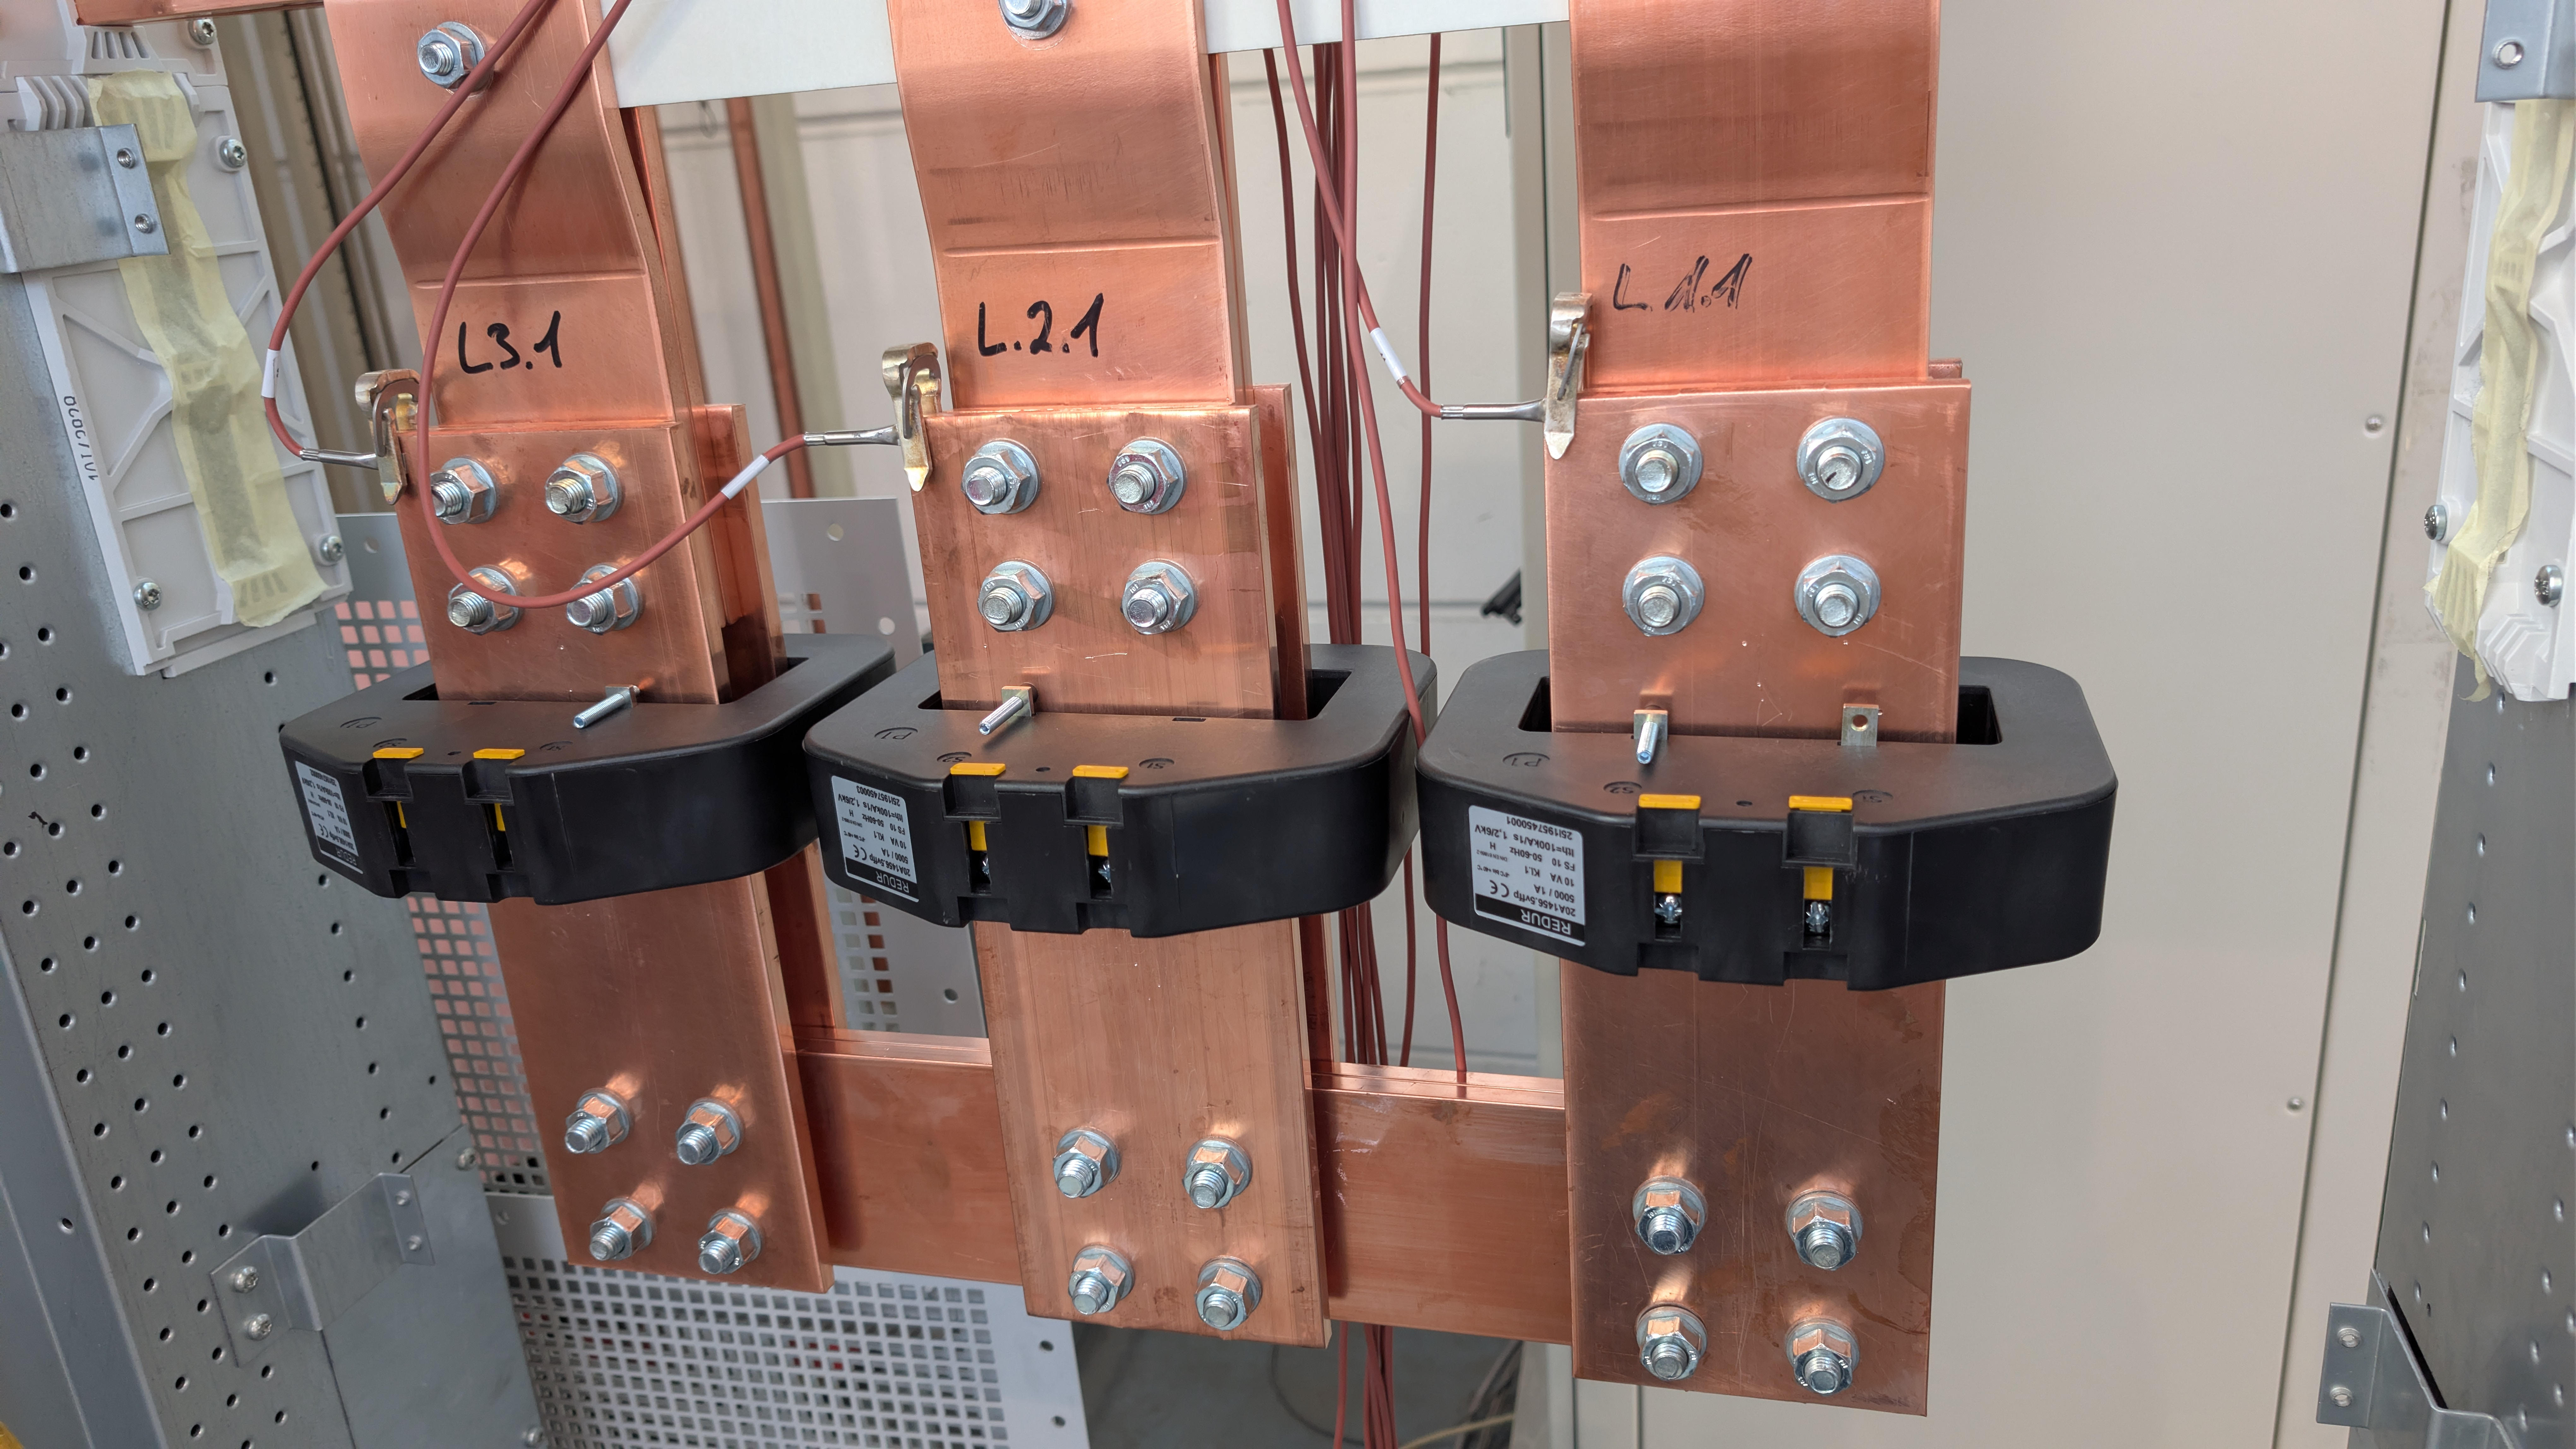
\includegraphics[width=1.0\textwidth]{03_Ressourcen/Bilder/kupferschienen_parallel.jpg}
    \caption{Versuchsaufbau in paralleler Schienenanordnung mit montiertem Messstromwandler}
    \label{pic:kupferschienen_parallel}
\end{figure}

\paragraph{Dreieckskonfiguration}
Für die Realisierung der Dreiecksanordnung wurde der Aufbau gemäß Abbildung~\ref{pic:kupferschienen_dreieck} modifiziert. Ein speziell gefertigter Kupferadapter führt hierbei die mittlere Phase L2 geometrisch aus der Ebene der Außenleiter heraus und versetzt die Schiene um \SI{140}{mm} nach vorne. Durch diesen Versatz spannen die Mittelpunkte der drei Leiter im Querschnitt ein Dreieck auf. 



Ziel dieser Anordnung ist eine symmetrischere Gestaltung der magnetischen Kopplung sowie die partielle Kompensation der vektoriellen Anteile der Fremdfelder im Bereich des Wandlerkerns. Auch in dieser Konfiguration wurden die ausgewählten Prüflinge vermessen.

\begin{figure}[H]
    \centering
    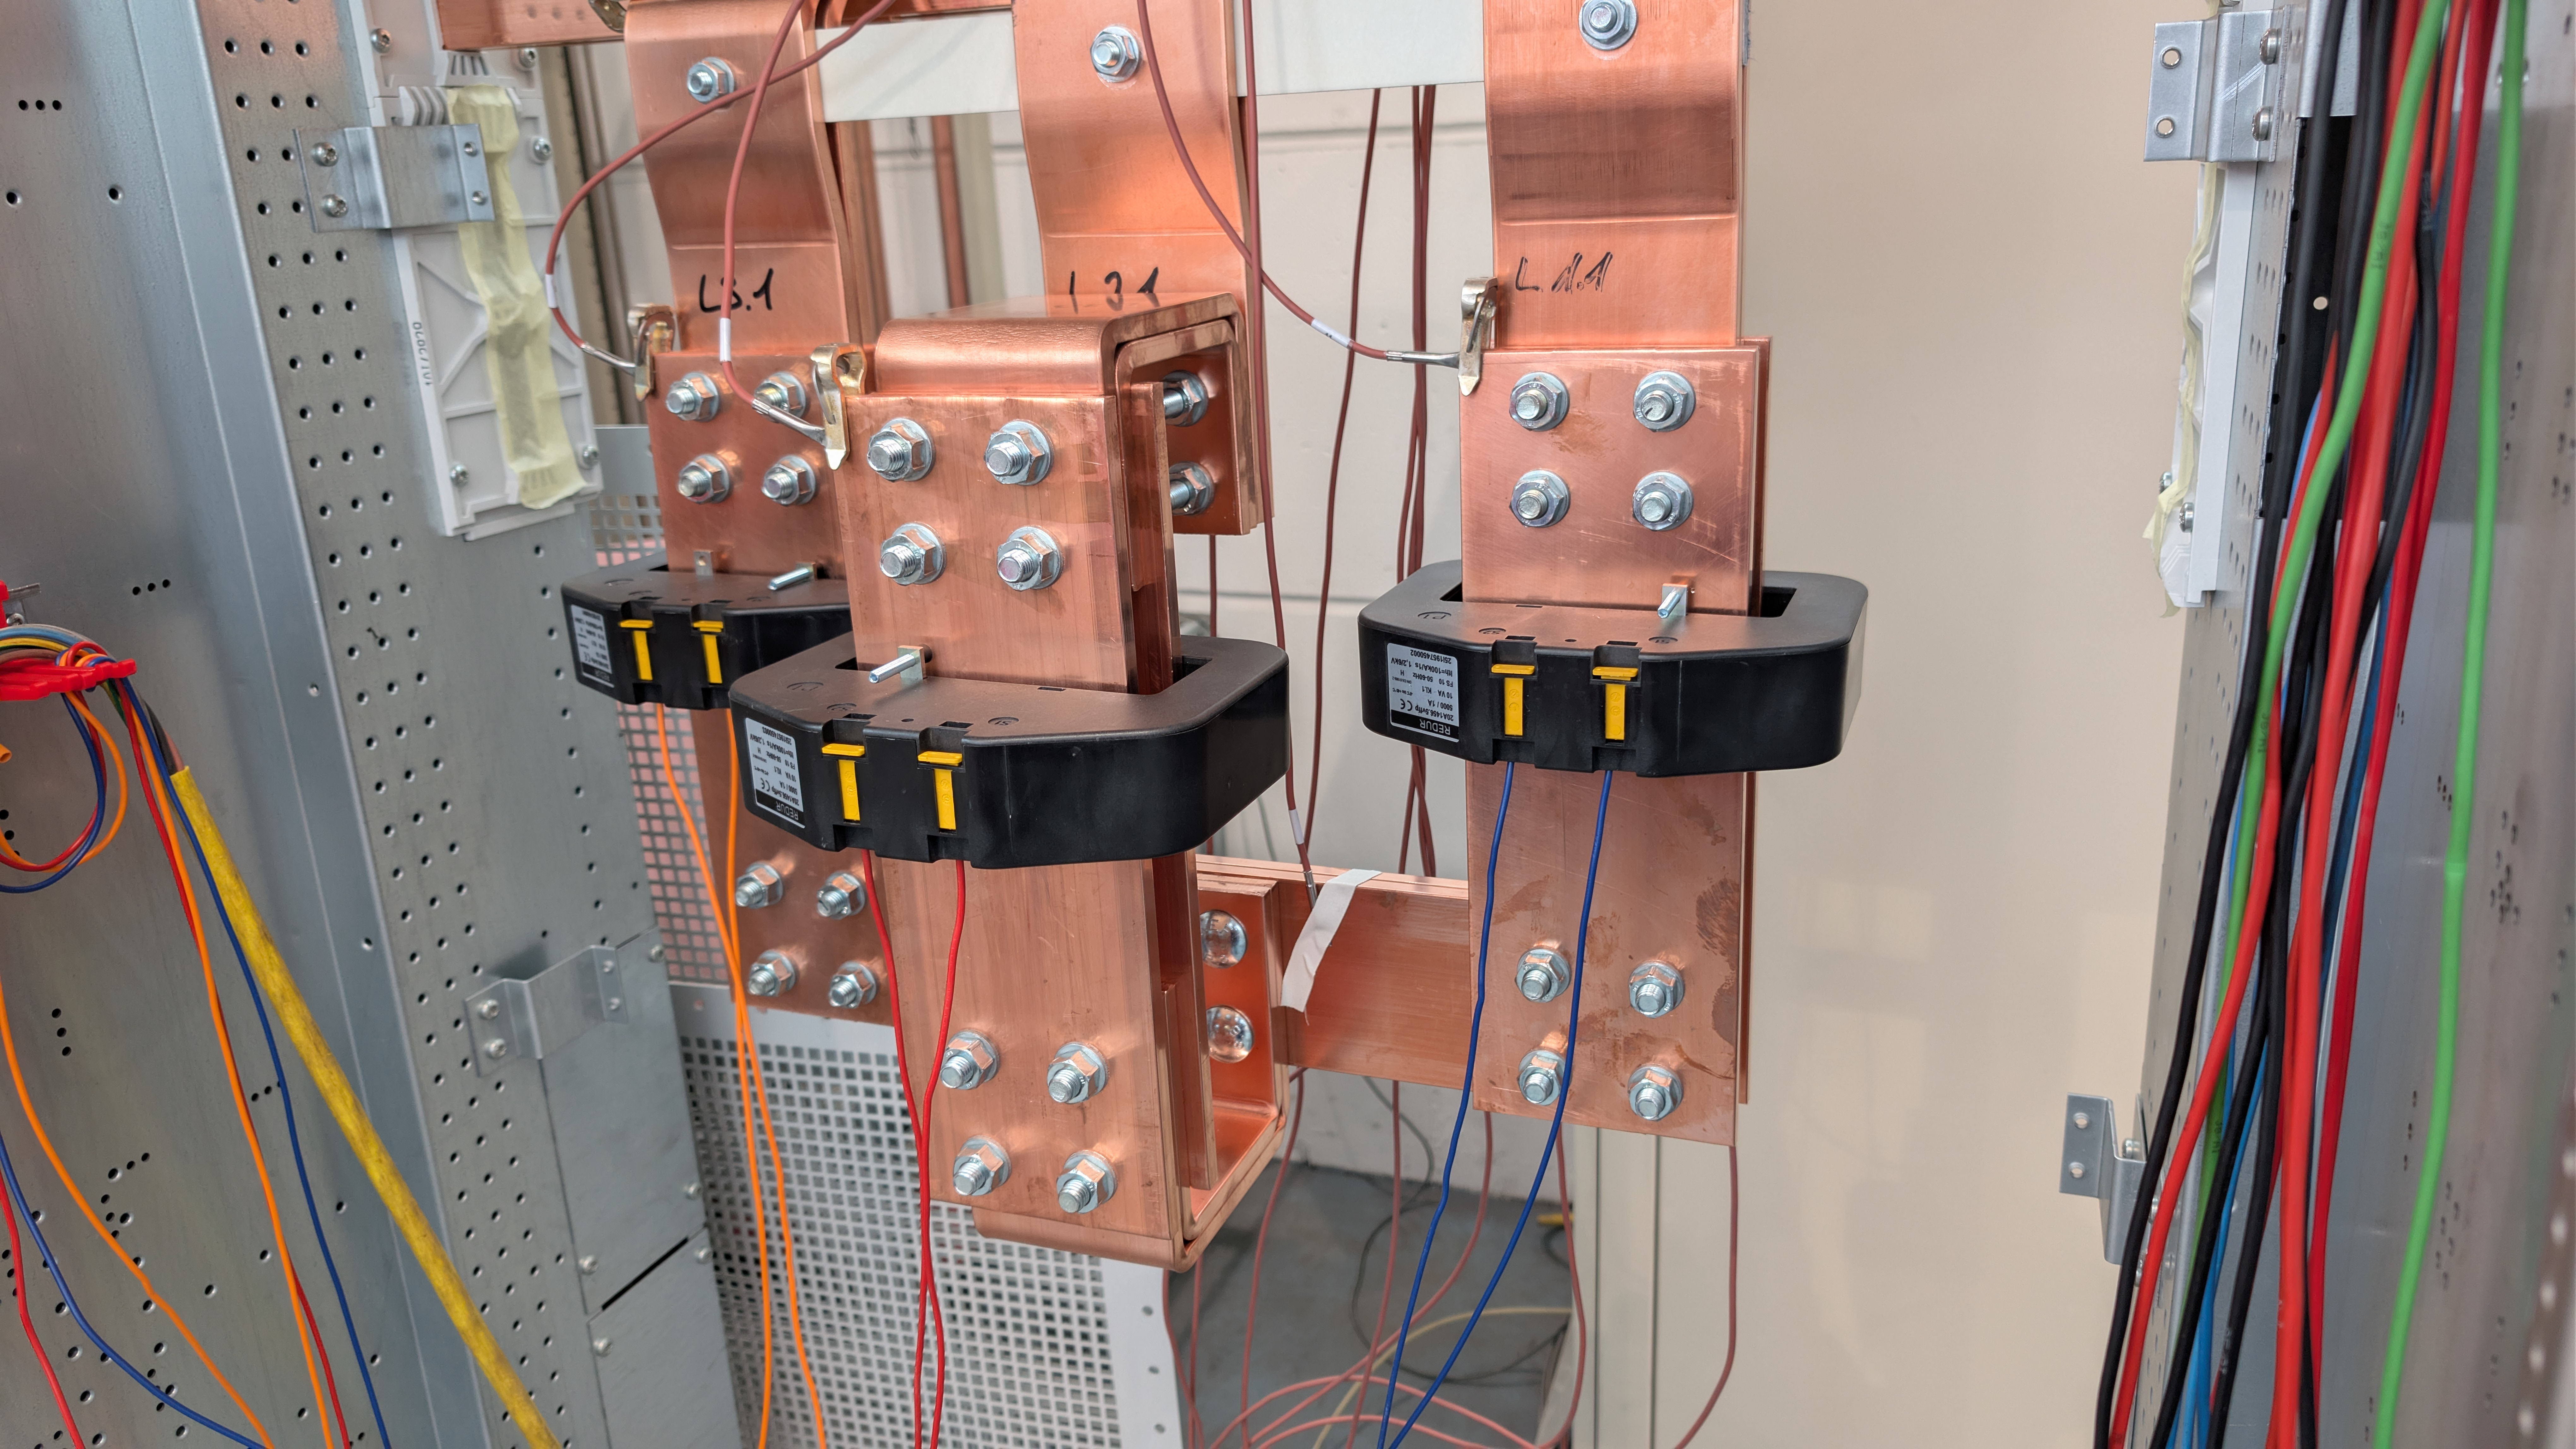
\includegraphics[width=1.0\textwidth]{03_Ressourcen/Bilder/kupferschienen_dreieck.jpg}
    \caption{Modifizierter Versuchsaufbau in Dreieckskonfiguration durch räumlichen Versatz der Phase L2 mittels Kupferadapter}
    \label{pic:kupferschienen_dreieck}
\end{figure}